\chapter{Visualization}
\label{cha:graphics}

\section{Overview}

{\opp} simulations can be run under graphical user interfaces (Tkenv,
Qtenv) that offer visualization and animation in addition to interactive
execution and other features. This chapter deals with model visualization.

{\opp} essentially provides three main tools for defining and enhancing
model visualization:

\begin{enumerate}

    \item \textit{Display strings} is the traditional way. It is a
    per-component string that encodes how the component (module or channel)
    will show up in the graphical user interface. Display strings can be
    specified in NED files, and can also be manipulated programmatically at
    runtime.

    \item \textit{The canvas.} The same user interface area that contains
    submodules and connections (i.e. the \textit{canvas}) can also display
    additional graphical elements that {\opp} calls \textit{figures}. Using
    figures, one can display lines, curves, polygons, images and text items,
    and anything that can be built by combining them and applying effects like
    rotation and scaling. Like display strings, figures can also be specified
    in NED files, but it is generally more useful to create and manipulate them
    programmatically. Extra canvas instances can also be created and populated
    at runtime.

    \item \textit{3D visualization} of the simulation's virtual world is a
    third possiblity. {\opp}'s 3D visualization capabilities come from the
    open-source OpenSceneGraph library and its osgEarth extension. These
    libraries offer high-level functionality, such as reading 3D model files
    directly from disk, or displaying maps, 3D terrain or Earth as a planet
    using online map and satellite imagery data sources.

\end{enumerate}

The following sections will cover the above topics in more detail, but first,
let us get acquainted with a new \cclass{cModule} virtual method that you
can redefine and place visualization-related code into.


\section{Placement of Visualization Code}
\label{sec:ch-graphics:refreshdisplay}

Traditionally, when C++ code was needed to enhance visualization, for
example to update a displayed status label or to refresh the position of a
mobile node, it was embedded in \ffunc{handleMessage()} functions, enclosed
in \ttt{if (ev.isGUI())} blocks. This was less than ideal, because the
visualization code would run for all events in that module and not just
before display updates when it was actually needed. In Express mode, for example,
Tkenv would only refresh the display once every second or so, during which
several hundred thousand or million events are processed, so visualization
code placed inside \ffunc{handleMessage()} could potentially waste a
significant amount of CPU cycles.

\subsection{The refreshDisplay() Method}

Starting from {\opp} version 5.0, visualization code can be placed into a
dedicated method. This method is called much more economically, that, only
when needed, i.e. only right before the GUI does a display update.

This method is called \ffunc{refreshDisplay()}, and is declared on
\cclass{cModule} as:

\begin{cpp}
virtual void refreshDisplay() const {}
\end{cpp}

Components that contain visualization-related code are expected to override
\ffunc{refreshDisplay()}, and move visualization code such as display string
manipulation, canvas figure maintenance and OSG scene graph updates into it.

When and how is \ffunc{refreshDisplay()} invoked? Strictly speaking, it is
undefined, but here are some hints:

\begin{enumerate}
\item It is invoked only under graphical user interfaces, currently Qtenv
     and Tkenv. It is not invoked under Cmdenv.

\item When invoked, it will be called on \textit{all} components of the
      simulation. It does not matter a module has a graphical inspector
      open or not.\footnote{This design decision simplifies the handling
      of cross-module visualization dependencies. Runtime overhead is
      still low, because display updates are practically only done at most
      a few times per second, never in a tight loop.}

\item It is invoked right before display updates. This includes the following:
      after network setup; in \textit{Step} and \textit{Run} modes after every event;
      in \textit{Fast} and \textit{Express} modes before each display update (they
      occur roughly once or a few times per second, thus, after processing
      a few tens, thousands or potentially millions of simulation events);
      after finalization.

\end{enumerate}

Here is an example of how one would use it:

\begin{cpp}
void FooModule::refreshDisplay() const
{
    // refresh statistics
    char buf[32];
    sprintf(buf, "Sent:%d  Rcvd:%d", numSent, numReceived);
    getDisplayString()->setTagArg("t", 0, buf);

    // update the mobile node's position
    Point pos = ...  // e.g. invoke a computePosition() method
    getDisplayString()->setTagArg("p", 0, pos.x);
    getDisplayString()->setTagArg("p", 1, pos.y);
}
\end{cpp}

\subsection{Advantages}

Overriding \ffunc{refreshDisplay()} has several advantages over putting the
simulation code into \ffunc{handleMessage()}. The first one is, as you have
probably guessed already, \textit{performance}. When running under Cmdenv,
the runtime cost of visualization code is literally zero, and when running
in \textit{Express} mode under Tkenv/Qtenv, it is practically zero because
the cost of one update is amortized over several hundred thousand or
million events.

The second advantage is also very practical: \textit{consistency} of the
visualization. If the simulation has cross-module dependencies such that
an event processed by one module affects the information displayed
by another module, with \ffunc{handleMessage()}-based visualization
the model may have inconsistent visualization until the second module
also processes an event and updates its displayed state. With
\ffunc{refreshDisplay()} this does not happen, because all modules
are refreshed together.

The third advantage is \textit{separation of concerns.} It is generally
not a good idea to intermix simulation logic with visualization code,
and \ffunc{refreshDisplay()} lets you completely separate the two.

\subsection{Why is \ffunc{refreshDisplay()} const?}

Code in \ffunc{refreshDisplay()} should never alter the state of the
simulation (mostly because from the simulation model's point of
view, it is completely unpredictable when and whether \ffunc{refreshDisplay()}
is invoked by the runtime), and the method is declared \ttt{const} to gently
encourage this behavior.

If visualization code makes use of internal caches or maintains some
other mutable state, such data members can be declared \ttt{mutable}
to allow \ffunc{refreshDisplay()} change them.


\section{Display Strings}
\label{sec:ch-graphics:display-strings}

Display strings\index{display strings} are compact textual descriptions
that specify the arrangement and appearance of representations of modules
in graphical user interfaces (currently Tkenv and Qtenv); they control how
the objects (compound modules, their submodules and connections) are
displayed. Display strings are specified in NED's \fprop{@display}
property, and can also be modified at runtime.

Display strings can be used in the following contexts:
\begin{itemize}
  \item \textit{submodules} -- display strings may contain position, arrangement
        (for module vectors), icon, icon color, auxiliary icon, status text,
        communication range (as circle or filled circle), tooltip, etc.
  \item \textit{compound modules, networks} -- display strings can specify
        background color, border color, border width,
        background image, scaling, grid, unit of measurement, etc.
  \item \textit{connections} -- display strings can specify positioning, color,
        line width, line style, text and tooltip
  \item \textit{messages} -- display strings can specify icon, icon color, etc.
\end{itemize}


\subsection{Syntax and Placement}

Display strings are specified in \fprop{@display} properties. The property
must contain a single string as value. The string should contain a
semicolon-separated list of tags. Each tag consists of a key, an equal sign
and a comma-separated list of arguments:

\begin{ned}
@display("p=100,100;b=60,10,rect,blue,black,2")
\end{ned}

Tag arguments may be omitted both at the end and inside the parameter list.
If an argument is omitted, a sensible default value is used. In the following
example, the first and second arguments of the \ttt{b} tag are omitted.

\begin{ned}
@display("p=100,100;b=,,rect,blue")
\end{ned}

Display strings can be placed in the \textit{parameters} section of module
and channel type definitions, and in submodules and connections. The
following NED sample illustrates the placement of display strings in the
code:

\begin{ned}
simple Server
{
    parameters:
        @display("i=device/server");
    ...
}

network Example
{
    parameters:
        @display("bgi=maps/europe");
    submodules:
        server: Server {
            @display("p=273,101");
        }
        ...
    connections:
        client1.out --> { @display("ls=red,3"); } --> server.in++;
}
\end{ned}

\subsection{Display String Inheritance}

At runtime, every module and channel object has one single display string object,
which controls its appearance in various contexts. The initial value of
this display string object comes from merging the \fprop{@display}
properties occurring at various places in NED files.
This section describes the rules for merging \fprop{@display} properties
to create the module or channel's display string.

\begin{itemize}
  \item Derived NED types inherit their display string from their base NED type.
  \item Submodules inherit their display string from their type.
  \item Connections inherit their display string from their channel type.
\end{itemize}

The base NED type's display string is merged into the current display string
using the following rules:

\begin{itemize}
  \item If a tag is present in the base display string, but not in the current one
        the whole tag (with all arguments) is added to the current display string.
        (e.g. base: \ttt{"i=icon,red"} current: \ttt{"p=2,4"} result: \ttt{"p=2,4;i=icon,red"})
  \item If a tag is present both in the base and in the current display string
        only tag arguments present in the base, but not in the current display string
        will be copied.
        (e.g. base: \ttt{"b=40,20"} current: \ttt{"b=,30,oval"} result: \ttt{"b=40,30,oval"})
  \item If the current display string contains a tag argument with value "-" (hyphen)
        that argument is treated as empty and will not be inherited from other
        display strings. Requesting the value of this argument will return its the
        default value.
  \item If neither the base display string nor the current one has value for a tag
        a suitable default value will be returned and used.
\end{itemize}

Example of display string inheritance:

\begin{ned}
simple Base {
    @display("i=block/queue"); // use a queue icon in all instances
}

simple Derived extends Base {
    @display("i=,red,60");  // ==> "i=block/queue,red,60"
}

network SimpleQueue {
    submodules:
        submod: Derived {
            @display("i=,yellow,-;p=273,101;r=70");
                     // ==> "i=block/queue,yellow;p=273,101;r=70"
        }
        ...
}
\end{ned}


\subsection{Display String Tags Used in Submodule Context}

The following tags define how a module appears on a graphical user interface
when viewed as a submodule:

\begin{itemize}
  \item \ttt{b} -- shape (box, oval, etc.)
  \item \ttt{i} -- icon
  \item \ttt{is} -- icon size
  \item \ttt{i2} -- auxiliary or status icon
  \item \ttt{p} -- positioning and layout
  \item \ttt{r} -- range indicator
  \item \ttt{q} -- queue information text
  \item \ttt{t} -- text
  \item \ttt{tt} -- tooltip
\end{itemize}

The following sections provide an overview and examples for each tag. More
detailed information, such as what each tag argument means, is available in
Appendix \ref{cha:display-string-tags}.

\subsubsection{Icons}

By default, modules are displayed with a simple default icon, but {\opp}
comes with a large set of categorized icons that you can choose from.
To see the what icons are available, look into the \ttt{images/} folder
in your {\opp} installation. The stock icons installed with {\opp} have
several size variants. Most of them have very small (vs), small (s),
large (l) and very large (vl) versions.

One can specify the icon with the \ttt{i} tag. The icon name should be
given with the name of the subfolder under \ttt{images/}, but without the
file name extension. The size is either as suffix of the icon name (e.g.
\ttt{\_l} for large), or can be specified separately with the \ttt{is} tag.

An example that displays the \textit{block/source} in large size:

\begin{ned}
@display("i=block/source;is=l");
\end{ned}

Icons may also be colorized, which can often be useful. Color can indicate
the status or grouping of the module, or simple serve aesthetic purposes.
The following example makes the icon 20\% red:

\begin{ned}
@display("i=block/source,red,20")
\end{ned}

\begin{center}
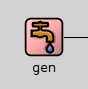
\includegraphics{figures/graphics-itag}
\end{center}

\subsubsection{Status Icon}

Modules may also display a small auxiliary icon in the top-right corner of
the main icon. This icon can be useful for displaying the status of the
module, for example, and can be set with the \ttt{i2} tag. Icons suitable
for use with \ttt{i2} are in the \ttt{status/} category.

An example:

\begin{ned}
@display("i=block/queue;i2=status/busy")
\end{ned}

\begin{center}

\includegraphics{figures/graphics-i2tag}
\end{center}

\subsubsection{Shapes}

To have a simple but resizable representation for your module, one can use
the \ttt{b} tag to create geometric shapes. Currently, \ttt{oval} and
\ttt{rectangle} are supported.

The following example displays an oval shape of size 70x30 with a 4-pixel
black border and red fill:

\begin{ned}
@display("b=70,30,oval,red,black,4")
\end{ned}

\begin{center}
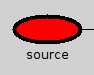
\includegraphics{figures/graphics-btag}
\end{center}

\subsubsection{Positioning}

The \ttt{p} tag allows one to define the position of a submodule or
otherwise affect its placement. If the \ttt{p} tag is missing or doesn't
specify the position, {\opp} will use a layouting algorithm to place the
module automatically.

The following example will place the module at the given position:

\begin{ned}
@display("p=50,79");
\end{ned}

\begin{note}
Coordinates and distances in \ttt{p}, \ttt{b} or \ttt{r} tags need not
be integers. Fractional numbers make sense because runtime GUIs (Tkenv,
Qtenv) support zooming.
\end{note}

If the submodule is a module vector, one can also specify in the \ttt{p}
tag how to arrange the elements of the vector. They can be arranged in a
row, a column, a matrix or a ring. The rest of the arguments in the \ttt{p}
tag depend on the layout type:

\begin{itemize}
  \item \ttt{row -- p=100,100,r,$deltaX$} (A row of modules with $deltaX$ units between the modules)
  \item \ttt{column -- p=100,100,c,$deltaY$} (A column of modules with $deltaX$ units between the modules)
  \item \ttt{matrix -- p=100,100,m,$noOfCols$,$deltaX$,$deltaY$} (A matrix with $noOfCols$ columns.
            $deltaX$ and $deltaY$ units between rows and columns)
  \item \ttt{ring -- p=100,100,ri,$rx$,$ry$} (A ring (oval) with $rx$ and $ry$ as the horizontal and vertical radius.)
  \item \ttt{exact (default) -- p=100,100,x,$deltaX$,$deltaY$} (Place each module at $(100+deltaX, 100+deltaY)$.
            The coordinates are usually set at runtime.)
\end{itemize}

A matrix layout for a module vector (note that the first two arguments, $x$
and $y$ are omitted, so the submodule matrix as a whole will be placed by
the layouter algorithm):

\begin{ned}
host[20]: Host {
    @display("p=,,m,4,50,50");
}
\end{ned}

\begin{figure}[htbp]
  \begin{center}
    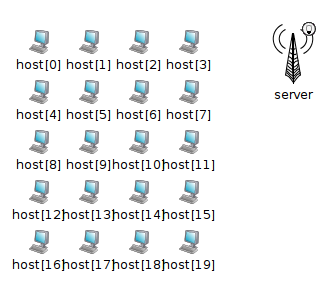
\includegraphics{figures/graphics-ptag}
    \caption{Matrix arrangement using the $p$ tag}
    \label{fig:graphics-ptag}
  \end{center}
\end{figure}

\subsubsection{Wireless Range}

In wireless simulations, it is often useful to be able to display a circle
or disc around the module to indicate transmission range, reception range,
or interference range. This can be done with the \ttt{r} tag.

The following example, the module will have circle with a 90-unit radius
around it as a range indicator:

\begin{ned}
submodules:
    ap: AccessPoint {
        @display("p=50,79;r=90");
    }
\end{ned}

\begin{figure}[htbp]
  \begin{center}
    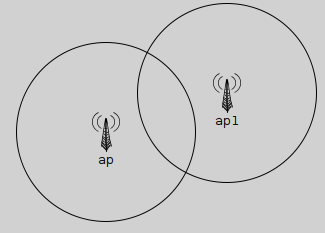
\includegraphics{figures/graphics-rtag}
    \caption{Range indicator using the $r$ tag}
    \label{fig:graphics-rtag}
  \end{center}
\end{figure}

\subsubsection{Queue Length}

If a module contains a queue object (\cclass{cQueue}), it is possible to
let the graphical user interface display the queue length next to the
module icon. To achieve that, specify the queue object's name (the string
set via the \ffunc{setName()} method) in the \ttt{q} display string tag.
{\opp} will find the queue object by traversing the object tree inside
the module.

For example, if the module contains a \cclass{cQueue} object named
\ttt{"jobQueue"}, you can can specify \ttt{q=jobQueue} in the display
string.

\begin{ned}
@display("q=jobQueue");
\end{ned}

\begin{center}
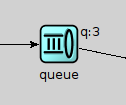
\includegraphics{figures/graphics-qtag}
\end{center}

\subsubsection{Text and Tooltip}

You can add a text description to any module using the \ttt{t}
(displayed along the module) or \ttt{tt} tag (displayed as a tooltip).
The following example displays a short text string along with the module
and adds a tooltip text string that can be seen by hovering over
them module with the mouse.

\begin{ned}
@display("t=Packets sent: 18;tt=Additional tooltip information");
\end{ned}

\begin{center}
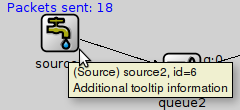
\includegraphics{figures/graphics-ttag}
\end{center}

\begin{note}
  The \ttt{t} and \ttt{tt} tags, when set at runtime, can be used to display
  various information about the module's state. The \ffunc{setTagArg()} method
  of \cclass{cDisplayString} can be used to update the text:

  \begin{cpp}
char buf[64];
sprintf(buf, "sent: %d, rcvd: %d", numPkSent, numPkReceived);
getDisplayString().setTagArg("t", 0, buf);
  \end{cpp}

\end{note}

For a detailed descripton of the display string tags, check
Appendix \ref{cha:display-string-tags}.

\subsection{Display String Tags Used in Module Background Context}

The following tags describe what a module looks like when opened in
a graphical user interface. They mostly deal with the module background.

\begin{itemize}
  \item \ttt{bgi} -- background image
  \item \ttt{bgtt} -- tooltip above the background
  \item \ttt{bgg} -- background grid
  \item \ttt{bgl} -- child layout
  \item \ttt{bgb} -- background size, color, border
  \item \ttt{bgu} -- measurement unit of coordinates/distances
\end{itemize}

In the following example, the background area is defined to be 6000x4500
units, and the map of Europe is used as a background, stretched to fill the
whole area. A grid is also drawn, with 1000 units between major ticks,
and 2 minor ticks per major tick.

\begin{ned}
network EuropePlayground
{
    @display("bgb=6000,4500;bgi=maps/europe,s;bgg=1000,2,grey95;bgu=km");
\end{ned}

\begin{figure}[htbp]
  \begin{center}
    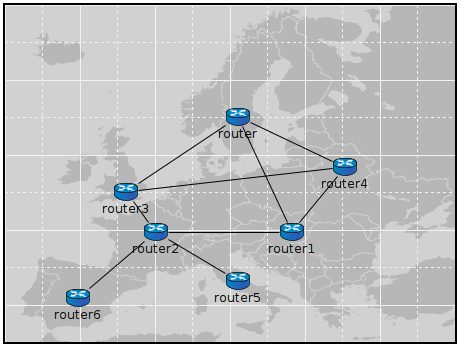
\includegraphics{figures/graphics-bgtags}
    \caption{Background image and grid}
    \label{fig:graphics-bgtags}
  \end{center}
\end{figure}

The \ttt{bgu} tag deserves special attention. It does not affect
the visual appearance, but instead it is a hint for model code
on how to interpret coordinates and distances in this compound
module. The above example specifies \ttt{bgs=km}, which means
that if the model attaches physical meaning to coordinates and
distances, then those numbers should be interpreted as kilometers.

More detailed information, such as what each tag argument means, is
available in Appendix \ref{cha:display-string-tags}.

\subsection{Connection Display Strings}

Connections may also have display strings. Connections inherit the
display string property from their channel types, in the same way as
submodules inherit theirs from module types. The default display
strings are empty.

Connections support the following tags:
\begin{itemize}
  \item{\ttt{ls} -- line style and color}
  \item{\ttt{t} -- text}
  \item{\ttt{tt} -- tooltip}
  \item{\ttt{m} -- orientation and positioning}
\end{itemize}

Example of a thick, red connection:
\begin{ned}
source1.out --> { @display("ls=red,3"); } --> queue1.in++;
\end{ned}

\begin{center}
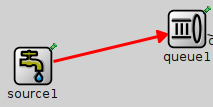
\includegraphics{figures/graphics-lstag}
\end{center}

\begin{note}
To hide a connection, specify zero line width in the display string:
\ttt{"ls=,0"}.
\end{note}

More detailed information, such as what each tag argument means, is
available in Appendix \ref{cha:display-string-tags}.

\subsection{Message Display Strings}

Message display strings affect how messages are shown during animation.
By default, they are displayed as a small filled circle, in one of
8 basic colors (the color is determined as \textit{message kind modulo 8}),
and with the message class and/or name displayed under it.
The latter is configurable in the Options dialog of Tkenv and Qtenv,
and message kind dependent coloring can also be turned off there.

\subsubsection{Specifying Message Display Strings}

Message objects do not store a display string by default, but you can redefine
the \cclass{cMessage}'s \ffunc{getDisplayString()} method and make it return
one.

Example of using an icon to represent a message:

\begin{cpp}
const char *CustomPacket::getDisplayString() const
{
    return "i=msg/packet;is=vs";
}
\end{cpp}

Alternatively, you can add the field \ffunc{displayString} to your message
definition (.msg file), and the message compiler will automatically generate
\ffunc{setDisplayString()} and \ffunc{getDisplayString()} methods for you:

\begin{msg}
message Job
{
    string displayString = "i=msg/package_s,kind";
...
\end{msg}

\subsubsection{Message Display String Tags}

The following tags can be used in message display strings:

\begin{itemize}
  \item \ttt{b} -- shape, color
  \item \ttt{i} -- icon
  \item \ttt{is} -- icon size
\end{itemize}

\begin{note}
   In message display strings, \ttt{kind} is accepted as a special color name.
   It will cause the color to be derived from \textit{message kind} field in the message.
\end{note}

The following example displays a small red box icon:

\begin{ned}
@display("i=msg/box,red;is=s");
\end{ned}

The next one displays a 15x15 rectangle, with while fill, and with a border
color dependent on the message kind:

\begin{ned}
@display("b=15,15,rect,white,kind,5");
\end{ned}

More detailed information, such as what each tag argument means, is
available in Appendix \ref{cha:display-string-tags}.


\subsection{Parameter Substitution}

Parameters of the module or channel containing the
display string can be substituted into the display string
with the \ttt{\$parameterName} notation:

Example:

\begin{ned}
simple MobileNode
{
    parameters:
        double xpos;
        double ypos;
        string fillColor;
        // get the values from the module parameters xpos,ypos,fillcolor
        @display("p=$xpos,$ypos;b=60,10,rect,$fillColor,black,2");
}
\end{ned}

\subsection{Colors}
\label{sec:ch-graphics:colors}

\subsubsection{Color Names}

A color may be given in several forms. One is English names: \ttt{blue},
\ttt{lightgrey}, \ttt{wheat}, etc.; the list includes all standard SVG
color names.

Another acceptable form is the HTML RGB syntax: \textit{\#rgb} or
\textit{\#rrggbb}, where \textit{r},\textit{g},\textit{b} are hex digits.

It is also possible to specify colors in HSB (hue-saturation-brightness) as
\textit{@hhssbb} (with \textit{h}, \textit{s}, \textit{b} being hex digits).
HSB makes it easier to scale colors e.g. from white to bright red.

You can produce a transparent background by specifying a hyphen (\textit{"-"})
as background color.

In message display strings, \ttt{kind} can also be used as a special color
name. It will map message kind to a color. (See the \ffunc{getKind()}
method of \cclass{cMessage}.)

\subsubsection{Icon Colorization}

The \ttt{"i="} display string tag allows for colorization of icons.
It accepts a target color and a percentage as the degree of colorization.
Percentage has no effect if the target color is missing.
Brightness of the icon is also affected -- to keep the original brightness,
specify a color with about 50\% brightness (e.g. \ttt{\#808080} mid-grey,
\ttt{\#008000} mid-green).

Examples:

\begin{itemize}
  \item \ttt{"i=device/server,gold"} creates a gold server icon
  \item \ttt{"i=misc/globe,\#808080,100"} makes the icon greyscale
  \item \ttt{"i=block/queue,white,100"} yields a "burnt-in" black-and-white icon
\end{itemize}

Colorization works with both submodule and message icons.


\subsection{Icons}
\label{sec:ch-graphics:icon-library}

\subsubsection{The Image Path}

In the current {\opp} version, module icons are PNG or GIF files. The icons shipped
with {\opp} are in the \ttt{images/} subdirectory. The IDE, Tkenv and Qtenv all
need the exact location of this directory to be able to load the icons.

Icons are loaded from all directories in the \textit{image path},
a semicolon-separated list of directories.
The default image path is compiled into Tkenv and Qtenv with the value
\ttt{"\textit{<omnetpp>}/\-images;./images"} -- which will work fine
as long as you don't move the directory, and you will also be able to
load more icons from the \ttt{images/} subdirectory of the current
directory. As users typically run simulation models from the model's
directory, this practically means that custom icons placed in the
\ttt{images/} subdirectory of the model's directory are automatically
loaded.

The compiled-in image path can be overridden with the \ttt{OMNETPP\_IMAGE\_PATH}
environment variable. The way of setting environment variables is system
specific: in Unix, if you are using the bash shell, adding a line

\begin{commandline}
export OMNETPP_IMAGE_PATH="$HOME/omnetpp/images;./images"
\end{commandline}

to \ttt{\textasciitilde/.bashrc} or \ttt{\textasciitilde/.bash\_profile} will do;
on Windows, environment variables can be set via the \textit{My Computer --> Properties} dialog.

You can extend the image path from \ffilename{omnetpp.ini} with the
\ttt{image-path} option, which is prepended to the environment
variable's value.

\begin{inifile}
[General]
image-path = "/home/you/model-framework/images;/home/you/extra-images"
\end{inifile}


\subsubsection{Categorized Icons}

Icons are organized into several categories, represented by folders.
These categories include:

\begin{itemize}
  \item \ttt{abstract/} - symbolic icons for various devices
  \item \ttt{background} - images useful as background, such as terrain map
  \item \ttt{block/} - icons for subcomponents (queues, protocols, etc).
  \item \ttt{device/} - network device icons: servers, hosts, routers, etc.
  \item \ttt{misc/} - node, subnet, cloud, building, town, city, etc.
  \item \ttt{msg/} - icons that can be used for messages
  \item \ttt{status/} - status icons such as up, down, busy, etc.
\end{itemize}

Icon names to be used with the \ttt{i}, \ttt{bgi} and other tags should
contain the subfolder (category) name but not the file extension. For
example, \ttt{/opt/omnetpp/images/block/sink.png} should be referred to as
\ttt{block/sink}.


\subsubsection{Icon Size}

Icons come in various sizes: normal, large, small, very small. Sizes are
encoded into the icon name's suffix: \ttt{\_vl}, \ttt{\_l}, \ttt{\_s}, \ttt{\_vs}.
In display strings, one can either use the suffix (\ttt{"i=device/router\_l"}),
or the \ttt{"is}" (\textit{icon size}) display string tag (\ttt{"i=device/router;is=l"}),
but not both at the same time (we recommend using the \ttt{is} tag.)

%The word "layouting" doesn't appear in the English dictionary, although it seems to appear
%  commonly in technical articles, etc. on the web. Up to this point, I have changed all
%  uses of layouting to layout, but I will leave it up to you to decide which one to use.
%  It sounds wrong to me, but it may be an acceptable usage in your particular domain.

\subsection{Layouting}
\label{sec:ch-graphics:layouting}

{\opp} implements an automatic layouting feature, using a variation of the
Spring Embedder algorithm. Modules which have not been assigned explicit
positions via the \ttt{"p="} tag will be automatically placed by the
algorithm.

Spring Embedder is a graph layouting algorithm based on a physical model.
Graph nodes (modules) repel each other like electric charges of the same
sign, and connections act as springs that pull nodes together. There is
also friction built in, in order to prevent oscillation of the nodes. The
layouting algorithm simulates this physical system until it reaches
equilibrium (or times out). The physical rules above have been slightly
tweaked to achieve better results.

The algorithm doesn't move any module which has fixed coordinates. Modules
that are part of a predefined arrangement (row, matrix, ring, etc., defined
via the 3rd and further args of the \ttt{"p="} tag) will be moved together,
to preserve their relative positions.

Caveats:

\begin{itemize}
  \item If the full graph is too big after layouting, it is scaled
    back so that it fits on the screen, \textit{unless it contains
    any fixed-position module}. (For obvious reasons: if there is a module
    with manually specified position, we don't want to move that one).
    To prevent rescaling, you can specify a sufficiently large bounding
    box in the background display string, e.g. \ttt{"b=2000,3000"}.
  \item Size is ignored by the present layouter, so modules with elongated
    shapes may not be placed ideally.
  \item The algorithm may produce erratic results, especially for small graphs
    when the number of submodules is small, or when using predefined
    (matrix, row, ring, etc) layouts. The "Re-layout" toobar button
    can then be very useful. Larger networks usually produce
    satisfactory results.
  \item The algorithm is starting from random positions.
     To get the best results you may experiment with
    different seeds by specifying them using the \ttt{bgl=\textit{seed}}
    display string tag.
\end{itemize}

\subsection{Changing Display Strings at Runtime}

It is often useful to manipulate the display string at runtime.
Changing colors, icon, or text may convey status change, and
changing a module's position is useful when simulating mobile
networks.

Display strings are stored in \cclass{cDisplayString} objects inside
channels, modules and gates. \cclass{cDisplayString} also lets you
manipulate the string.

As far as \cclass{cDisplayString} is concerned, a display string
(e.g. \ttt{"p=100,125;i=cloud"}) is a string that consist of several
\textit{tags} separated by semicolons, and each tag has a \textit{name}
and after an equal sign, zero or more \textit{arguments} separated by commas.

The class facilitates tasks such as finding out what tags a display string
has, adding new tags, adding arguments to existing tags, removing tags or
replacing arguments. The internal storage method allows very fast
operation; it will generally be faster than direct string manipulation. The
class doesn't try to interpret the display string in any way, nor does it
know the meaning of the different tags; it merely parses the string as data
elements separated by semicolons, equal signs and commas.

To get a pointer to a \cclass{cDisplayString} object, you can call
the components's \ffunc{getDisplayString()} method.

\begin{note}
The connection display string is stored in the channel object, but it
can also be accessed via the source gate of the connection.
\end{note}

The display string can be overwritten using the \ffunc{parse()} method.
Tag arguments can be set with \ffunc{setTagArg()}, and tags removed
with \ffunc{removeTag()}.

The following example sets a module's position, icon and status icon
in one step:

\begin{cpp}
cDisplayString& dispStr = getDisplayString();
dispStr.parse("p=40,20;i=device/cellphone;i2=status/disconnect");
\end{cpp}

Setting an outgoing connection's color to red:

\begin{cpp}
cDisplayString& connDispStr = gate("out")->getDisplayString();
connDispStr.parse("ls=red");
\end{cpp}

Setting module background and grid with background display string tags:

\begin{cpp}
cDisplayString& parentDispStr = getParentModule()->getDisplayString();
parentDispStr.parse("bgi=maps/europe;bgg=100,2");
\end{cpp}

The following example updates a display string so that it contains
the \ttt{p=40,20} and \ttt{i=device/cellphone} tags:

\begin{cpp}
dispStr.setTagArg("p", 0, 40);
dispStr.setTagArg("p", 1, 20);
dispStr.setTagArg("i", 0, "device/cellphone");
\end{cpp}

\section{Bubbles}

Modules can display a transient bubble with a short message (e.g. "Going
down" or "Connection estalished") by calling the \ffunc{bubble()} method of
\cclass{cComponent}. The method takes the string to be displayed as a
\ttt{const char *} pointer.

An example:
\begin{cpp}
bubble("Going down!");
\end{cpp}

\begin{center}
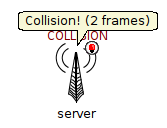
\includegraphics{figures/graphics-bubble}
\end{center}

If the module often displays bubbles, it is recommended to make the
corresponding code conditional on \ffunc{hasGUI()}. \ffunc{hasGUI()}
returns \textit{false} if the simulation is running under Cmdenv.

\begin{cpp}
if (hasGUI()) {
    char text[32];
    sprintf(text, "Collision! (%s frames)", numCollidingFrames);
    bubble(text);
}
\end{cpp}



\section{The Canvas}
\label{sec:ch-graphics:canvas}

\subsection{Overview}

The canvas is the 2D drawing API of {\opp}. Using the canvas, one can
display lines, curves, polygons, images, text items and their combinations,
using colors, transparency, geometric transformations, antialiasing and
more. Drawings created with the canvas API can be viewed when the simulation
is run under a graphical user interface (Tkenv or Qtenv).

Use cases for the canvas API include displaying textual annotations,
status information, live statistics in the form of plots, charts, gauges,
counters, etc. Other types of simulations may call for different types of
graphical presentation. For example, in mobile and wireless simulations,
the canvas API can be used to draw the scene including a background (like a
street map or floor plan), mobile objects (vehicles, people), obstacles
(trees, buildings, hills), antennas with orientation, and also extra
information like connectivity graph, movement trails, individual
transmissions and so on.

An arbitrary number of drawings (canvases) can be created, and every module
already has one by default. A module's default canvas is the one on which
the module's submodules and internal connections are also displayed, so the
canvas API can be used to enrich the default, display string based
presentation of a compound module.

{\opp} calls the items that appear on a canvas \textit{figures}. The
corresponding C++ types are \cclass{cCanvas} and \cclass{cFigure}. In fact,
\cclass{cFigure} is an abstract base class, and different kinds of figures
are represented by various subclasses of \cclass{cFigure}.

Figures can be declared statically in NED files using \fprop{@figure}
properties, and can also be accessed, created and manipulated
programmatically at runtime.


\subsection{Creating, Accessing and Viewing Canvases}

A canvas is represented by the \cclass{cCanvas} C++ class. A module's
default canvas can be accessed with the \ffunc{getCanvas()} method of
\cclass{cModule}. For example, a toplevel submodule can get hold of the
network's canvas with the following line:

\begin{cpp}
cCanvas *canvas = getParentModule()->getCanvas();
\end{cpp}

Using the canvas pointer, it is possible to check what figures it
contains, add new figures, manipulate existing ones, and so on.

New canvases can be created by simply creating new \cclass{cCanvas}
objects, like so:

\begin{cpp}
cCanvas *canvas = new cCanvas("liveStatistics"); // arbitrary name string
\end{cpp}

To view the contents of these additional canvases in Tkenv or Qtenv, one
needs to navigate to the canvas' owner object (which will usually be the
module that created the canvas), view the list of objects it contains, and
double-click the canvas in the list. Giving meaningful names to extra
canvas objects like in the example above can simplify the process of
locating them in the Tkenv/Qtenv GUI.


\subsection{Figure Classes}

The base class of all figure classes is \cclass{cFigure}. The class hierarchy
is shown below.

\begin{figure}[htbp]
  \begin{center}
    \includegraphics{figures/figure-inheritance}
    \caption{cFigure class hierarchy}
  \end{center}
\end{figure}

In subsequent sections, we'll first describe features that are common
to all figures, then we'll briefly cover each figure class. Finally,
we'll look into how one can define new figure types.

\begin{note}
Figures are only data storage classes. The real drawing code is inside
Tkenv/Qtenv; it might involve a parallel data structure, figure renderer classes, etc.
When an inspector is not open, these things don't exist. Therefore, data flow
is only one-directional -- figures affect the rendered image, but figures
cannot access e.g. the actual bounding box of a text just drawn.
\end{note}


\subsection{Figure Hierarchy}

Figures on a canvas form a hierarchy. The canvas has a \textit{root
figure}, and all toplevel figures in the canvas are children of the root
figure. In addition, any figure may contain further figures as children.
(That is, \textit{child list} is the built-in property of \cclass{cFigure},
not of a specific subclass like \cclass{cGroupFigure}.)

Every figure also has a name string, inherited from \cclass{cNamedObject}.
Putting it together with the figure hierarchy, this means that every figure
also has a \textit{hierarchical name}. It consists of the names of figures
in the path from the root figure down to the the figure, joined with dots.
(The name of the root figure itself is omitted.)

You can get the root figure of the canvas with the \ffunc{getRootFigure()}
member function, but that is usually unnecessary, because the
\cclass{cCanvas}, like \cclass{cFigure}, has methods for accessing and
manipulating its child figures directly.

You can add a child figure \ffunc{addFigure()}. It has two flavours: one
for appending, and one for inserting at a numeric position. The order of
children is important because it also denotes Z-order. Z-order comes into
play when children are overlapping on the screen: the first child will be
the bottom-most one, and the last child will be the topmost one (think of
it like drawing order). The methods \ffunc{addFigureAbove()} and
\ffunc{addFigureBelow()} allows one to insert a figure into the child list
relative to an existing child figure.

Child figures can be accessed by name (\ffunc{getFigure(name)}), or
enumerated by index in the child list (\ffunc{getFigure(k)},
\ffunc{getNumFigures()}). You can obtain the index of a child figure using
\ffunc{findFigure()}.

The following code illustrates these methods:

\begin{cpp}
// print the names of child figures above "cloud" in Z-order
// (in the code, 'parent' can be either a canvas or a figure):
cFigure *cloudFigure = parent->getFigure("cloud");
if (cloudFigure) {
    int cloudPos = parent->findFigure(cloudFigure);
    for (int i = cloudPos+1; i < parent->getNumFigures(); i++)
        EV << parent->getFigure(i)->getName() << endl;
}
\end{cpp}

It is also possible to locate a figure by its hierarchical name
(\ffunc{getFigureByPath()}), and to find figure by its (non-hierarchical)
name anywhere in a figure subtree (\ffunc{findFigureRecursively()}).

To remove a figure from the child list, use \ffunc{removeFigure()} with
either the figure's pointer or its index in the child list.

The \ffunc{dup()} method of figure classes only duplicates the very figure
on which it was called. To clone a figure including children, use the
\ffunc{dupTree()} method.


\subsection{Creating and Manipulating Figures from NED and C++}

As mentioned earlier, figures can be defined in the NED file, so they
don't always need to be created programmatically. This possibility is
useful for creating static backgrounds or statically defining placeholders
for dinamically displayed items, among others. Figures defined from NED can
be accessed and manipulated from C++ code in the same way as dynamically
created ones.

Figures are defined in NED by adding \fprop{@figure} properties to a module definition.
The hierarchical name of the figure goes into the property index, that is, in
square brackets right after \ttt{@figure}. The parent of the figure must
already exist, that is, when defining \ttt{foo.bar.baz}, both \ttt{foo} and
\ttt{foo.bar} must have already been defined (in NED).

Type and various attributes of the figure go into property body, as
\textit{key-valuelist} pairs. \ttt{type=line} creates a
\cclass{cLineFigure}, \ttt{type=rectangle} creates a
\cclass{cRectangleFigure}, \ttt{type=text} creates a \cclass{cTextFigure},
and so on; the list of accepted types is given in appendix
\ref{cha:figure-definitions}. Further attributes largely correspond to
getters and setters of the C++ class denoted by the \ttt{type} attribute.

The following example creates a green rectangle and the text
\textit{"placeholder"} in it in NED, and the subsequent C++ code changes
the same text to \textit{"Hello World!"}.

NED part:

\begin{ned}
module Foo
{
    @display("bgb=800,500");
    @figure[box](type=rectangle; coords=10,50; size=200,100; fillColor=green);
    @figure[box.txt](type=text; coords=20,80; text=placeholder);
}
\end{ned}

And the C++ part:

\begin{cpp}
// we assume this code runs in a submodule of the above "Foo" module
cCanvas *canvas = getParentModule()->getCanvas();

// obtain the figure pointer by hierarchical name, and change the text:
cTextFigure *textFigure = dynamic_cast<cTextFigure *>(
                              canvas->getFigureByPath("box.txt"));
textFigure->setText("Hello World!");
\end{cpp}

%% In addition to \ttt{type}, there are some more special attributes
%% (\ttt{visible}, \ttt{tags}, \ttt{transform}, \ttt{childZ})



\subsection{Transforms}

One of the most powerful features of the Canvas API is being able to assign
geometric transformations to figures. {\opp} uses 2D homogeneous
transformation matrices, which are able to express affine transforms such
as translation, scaling, rotation and skew (shearing). The
transformation matrix used by {\opp} has the following format:

\[ T = \left( \begin{array}{ccc}
a & c & t_1 \\
b & d & t_2 \\
0 & 0 & 1 \end{array} \right)\]

In a nutshell, given a point with its $(x, y)$ coodinates, one can obtain the
transformed version of it by multiplying the transformation matrix by the
$(x \ y \ 1)$ column vector (a.k.a. homogeneous coordinates), and dropping the
third component:

\[ \left( \begin{array}{c} x' \\ y' \\ 1 \end{array} \right)
 = \left( \begin{array}{ccc}
a & c & t_1 \\
b & d & t_2 \\
0 & 0 & 1 \end{array} \right)
\left( \begin{array}{c} x \\ y \\ 1 \end{array} \right)
\]

The result is the point $(ax+cy+t_1, bx+dy+t_2)$. As one can deduce, $a$,
$b$, $c$, $d$ are responsible for rotation, scaling and skew, and $t_1$ and
$t_2$ for translation. Also, transforming a point by matrix $T_1$ and then by
$T_2$ is equivalent to transforming the point by the matrix $T_2 T_1$ due to
the associativity of matrix multiplication.


\subsubsection{The Transform Class}

Transformation matrices are represented in {\opp} by the \cclass{cFigure::Transform}
class.

A \cclass{cFigure::Transform} transformation matrix can be initialized in
several ways. First, it is possible to assign its \ttt{a}, \ttt{b},
\ttt{c}, \ttt{d}, \ttt{t1}, \ttt{t2} members directly (they are public), or
via a six-argument constructor. However, it is usually more convenient to
start from the identity transform (as created by the default constructor), and
invoke one or more of its several \ffunc{scale()}, \ffunc{rotate()},
\ffunc{skewx()}, \ffunc{skewy()} and \ffunc{translate()} member functions.
They update the matrix to (also) perform the given operation (scaling,
rotation, skewing or translation), as if left-multiplied by a temporary
matrix that corresponds to the operation.

The \ffunc{multiply()} method lets you chain transformations: \ttt{t1.multiply(t2)}
sets \ttt{t1} to the product \ttt{t2*t1}.

To transform a point (represented by the class \cclass{cFigure::Point}),
one can use the \ffunc{applyTo()} method of \cclass{Transform}.

The following code fragment should clarify this:

\begin{cpp}
// allow Transform and Point to be referenced without the cFigure:: prefix
typedef cFigure::Transform Transform;
typedef cFigure::Point Point;

// create a matrix that scales by 2, rotates by 45 degrees, and translates by (100,0)
Transform t = Transform().scale(2.0).rotate(M_PI/4).translate(100,0);

// apply the transform to the point (10, 20)
Point p(10, 20);
Point p2 = t.applyTo(p);
\end{cpp}


\subsubsection{Figure Transforms}

Every figure has an associated transformation matrix, which
affects how the figure and its figure subtree are displayed.
In other words, the way a figure displayed is affected by its own
transformation matrix and the transformation matrices of all of its
ancestors, up to the root figure of the canvas. The effective transform
will be the product of those transformation matrices.

A figure's transformation matrix is directly accessible via \cclass{cFigure}'s
\ffunc{getTransform()}, \ffunc{setTransform()} member functions.
For convenience, \cclass{cFigure} also has several \ffunc{scale()}, \ffunc{rotate()},
\ffunc{skewx()}, \ffunc{skewy()} and \ffunc{translate()} member functions,
which directly operate on the internal transformation matrix.

Some figures have visual aspects that are not, or only optionally affected
by the transform. For example, the size and orientation of the text
displayed by \cclass{cLabelFigure}, in contrast to that of
\cclass{cTextFigure}, is unaffected by transforms (and of manual zoom as
well). Only position is transformed.

\subsubsection{Transform vs move()}

In addition to the \ffunc{translate()}, \ffunc{scale()}, \ffunc{rotate()},
etc. functions that update the figure's transformation matrix, figures also
have a \ffunc{move()} method. \ffunc{move()}, like \ffunc{translate()},
also moves the figure by a $dx$, $dy$ offset. However, \ffunc{move()} works
by changing the figure's coordinates, and not by changing the
transformation matrix.

Since every figure class stores and interprets its position differently,
\ffunc{move()} is defined for each figure class independently. For example,
\cclass{cPolylineFigure}'s \ffunc{move()} changes the coordinates of each point.

\ffunc{move()} is recursive, that is, it not only moves the figure on which
it was called, but also its children. There is also a non-recursive variant,
called \ffunc{moveLocal()}.


\subsection{Showing/Hiding Figures}

\subsubsection{Visibility Flag}

Figures have a visibility flag that controls whether the figure is
displayed. Hiding a figure via the flag will hide the whole figure subtree,
not just the figure itself. The flag can be accessed via the
\ffunc{isVisible()}, \ffunc{setVisible()} member functions of
\cclass{cFigure}.


\subsubsection{Tags}

Figures can also be assigned a number of textual tags. Tags do not directly
affect rendering, but graphical user interfaces that display canvas
content, namely Tkenv and Qtenv, offer functionality to interactively
show/hide figures based on tags they contain. This GUI figure filter allows
one to express conditions like \textit{"Show only figures that have tag
\ttt{foo} or \ttt{bar}, but among them, hide those that also contain
tag \ttt{baz}".} Tag-based filtering and the visibility flag are in AND
relationship -- figures hidden via \ttt{setVisible(false)} cannot be
displayed using tags. Also when a figure is hidden using the tag filter,
its figure subtree will also be hidden.

The tag list of a figure can be accessed with the \ffunc{getTags()} and
\ffunc{setTags()} \cclass{cFigure} methods; they return/accept a single
string that contains the tags separated by spaces (a tag itself cannot
contain a space.)

Tags functionality, when used carefully, allows one to define "layers"
that can be turned on/off from Tkenv/Qtenv.

%% TODO example

\subsection{Specifying Positions, Colors, Fonts and Other Properties}

\subsubsection{Points}

Points are represented by the \cclass{cFigure::Point} struct:

\begin{cpp}
struct Point {
    double x, y;
    ...
};
\end{cpp}

In addition to the public \ttt{x}, \ttt{y} members and a two-argument
constructor for convenient initialization, the struct provides overloaded
operators (+,-,*,/) and some utility functions like \ffunc{translate()},
\ffunc{distanceTo()} and \ffunc{str()}.

\subsubsection{Rectangles}

Rectangles are represented by the \cclass{cFigure::Rectangle} struct:

\begin{cpp}
struct Rectangle {
    double x, y,
    double width, height;
    ...
};
\end{cpp}

A rectangle is specified with the coordinates of their top-left corner,
their width and height. The latter two are expected to be nonnegative. In
addition to the public \ttt{x}, \ttt{y}, \ttt{width}, \ttt{height} members
and a four-argument constructor for convenient initialization, the struct
also has utility functions like \ffunc{getCenter()}, \ffunc{getSize()},
\ffunc{translate()} and \ffunc{str()}.

\subsubsection{Colors}

Colors are represented by the \cclass{cFigure::Color} struct as 24-bit RGB colors:

\begin{cpp}
struct Color {
    uint8_t red, green, blue;
    ...
};
\end{cpp}

In addition to the public \ttt{red}, \ttt{green}, \ttt{blue} members
and a three-argument constructor for convenient initialization, the struct
also has a string-based constructor and \ffunc{str()} function.

The string form accepts various notations: HTML colors (\ttt{\#rrggbb}),
HSB colors in a similar notation (\ttt{@hhssbb}), and English color names
(SVG and X11 color names, to be more precise.)

However, one doesn't need to use \cclass{Color} directly.
There are also predefined constants for the basic colors (\ttt{BLACK},
\ttt{WHITE}, \ttt{GREY}, \ttt{RED}, \ttt{GREEN}, \ttt{BLUE}, \ttt{YELLOW},
\ttt{CYAN}, \ttt{MAGENTA}), as well as a collection of carefully chosen
dark and light colors, suitable for e.g. chart drawing, in the arrays
\ttt{GOOD\_DARK\_COLORS[]} and \ttt{GOOD\_LIGHT\_COLORS[]}; for convenience,
the number of colors in each are in the \ttt{NUM\_GOOD\_DARK\_COLORS}
and \ttt{NUM\_GOOD\_LIGHT\_COLORS} constants).

The following ways of specifying colors are all valid:

\begin{cpp}
cFigure::BLACK;
cFigure::Color("steelblue");
cFigure::Color("#3d7a8f");
cFigure::Color("@20ff80");
cFigure::GOOD_DARK_COLORS[2];
cFigure::GOOD_LIGHT_COLORS[intrand(NUM_GOOD_LIGHT_COLORS)];
\end{cpp}


\subsubsection{Fonts}

The requested font for text figures is represented by the \cclass{cFigure::Font}
struct. It stores the typeface, font style and font size in one.

\begin{cpp}
struct Font {
    std::string typeface;
    int pointSize;
    uint8_t style;
    ...
};
\end{cpp}

The font does not need to be fully specified, there are some defaults. When
\ttt{typeface} is set to the empty string or when \ttt{pointSize} is zero
or a negative value, that means that the default font or the default size
should be used, respectively.

The \ttt{style} field can be either \ttt{FONT\_NONE}, or the binary OR of
the following constants: \ttt{FONT\_BOLD}, \ttt{FONT\_ITALIC},
\ttt{FONT\_UNDERLINE}.

The struct also has a three-argument constructor for convenient
initialization, and an \ffunc{str()} function that returns a human-readable
text representation of the contents.

Some examples:

\begin{cpp}
cFigure::Font("Arial");  // default size, normal
cFigure::Font("Arial", 12);  // 12pt, normal
cFigure::Font("Arial", 12, cFigure::FONT_BOLD | cFigure::FONT_ITALIC);
\end{cpp}


\subsubsection{Other Line and Shape Properties}

\cclass{cFigure} also contains a number of enums as inner types to describe
various line, shape, text and image properties. Here they are:

\tbf{LineStyle}

Values: \ttt{LINE\_SOLID}, \ttt{LINE\_DOTTED}, \ttt{LINE\_DASHED}

This enum (\cclass{cFigure::LineStyle}) is used by line and shape figures
to determine their line/border style. The precise graphical interpretation,
e.g. dash lengths for the \textit{dashed} style, depends on the graphics
library that the GUI was implemented with.

\tbf{CapStyle}

Values: \ttt{CAP\_BUTT}, \ttt{CAP\_ROUND}, \ttt{CAP\_SQUARE}

This enum is used by line and path figures, and it indicates the shape to
be used at the end of the lines or open subpaths.

\begin{center}
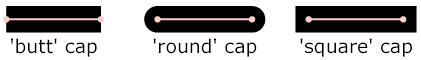
\includegraphics[scale=0.8]{figures/graphics-linecaps}
\end{center}

\tbf{JoinStyle}

Values: \ttt{JOIN\_BEVEL}, \ttt{JOIN\_ROUND}, \ttt{JOIN\_MITER}

This enum indicates the shape to be used when two line segments are joined,
in line or shape figures.

\begin{center}

\includegraphics[scale=0.8]{figures/graphics-linejoins}
\end{center}

\tbf{FillRule}

Values: \ttt{FILL\_EVENODD}, \ttt{FILL\_NONZERO}.

This enum determines which regions of a self-intersecting shape
should be considered to be inside the shape, and thus be filled.

\begin{center}

\includegraphics[scale=0.8]{figures/graphics-fillrule}
\end{center}

\tbf{Arrowhead}

Values: \ttt{ARROW\_NONE}, \ttt{ARROW\_SIMPLE}, \ttt{ARROW\_TRIANGLE}, \ttt{ARROW\_BARBED}.

Some figures support displaying arrowheads at one or both ends of a line.
This enum determines the style of the arrowhead to be used.

\begin{center}

\includegraphics[scale=0.8]{figures/graphics-arrowheads}
\end{center}

\tbf{Interpolation}

Values: \ttt{INTERPOLATION\_NONE}, \ttt{INTERPOLATION\_FAST}, \ttt{INTERPOLATION\_BEST}.

Interpolation is used for rendering an image when it is not displayed at
its native resolution. This enum indicates the algorithm to be used for
interpolation.

The mode \textit{none} selects the "nearest neighbor" algorithm.
\textit{Fast} emphasizes speed, and \textit{best} emphasizes quality;
however, the exact choice of algorithm (bilinear, bicubic, quadratic, etc.)
depends on features of the graphics library that the GUI was implemented with.

\tbf{Anchor}

Values:
\ttt{ANCHOR\_CENTER}, \ttt{ANCHOR\_N}, \ttt{ANCHOR\_E}, \ttt{ANCHOR\_S}, \ttt{ANCHOR\_W},
\ttt{ANCHOR\_NW}, \ttt{ANCHOR\_NE}, \ttt{ANCHOR\_SE}, \ttt{ANCHOR\_SW};
\ttt{ANCHOR\_BASELINE\_START}, \ttt{ANCHOR\_BASELINE\_MIDDLE}, \\ \ttt{ANCHOR\_BASELINE\_END}.

Some figures like text and image figures are placed by specifying a single
point (\textit{position}) plus an anchor mode, a value from this enum. The
anchor mode indicates which point of the bounding box of the figure should
be positioned over the specified point. For example, when using
\ttt{ANCHOR\_N}, the figure is placed so that its top-middle point falls at
the specified point.

The last three, \textit{baseline} constants are only used with text
figures, and indicate that the start, middle or end of the text's baseline
is the anchor point.


\subsection{cLineFigure and Other Figure Classes}

Now that we know all about figures in general, we can look into specific
figure classes.

\subsubsection{cAbstractLineFigure}

\cclass{cAbstractLineFigure} is the common base class for various line
figures, providing line color, style, width, opacity, arrowhead and other
properties for them.

Line color can be set with \ffunc{setLineColor()}, and line width with
\ffunc{setLineWidth()}. Lines can be solid, dashed, dotted, etc.; line
style can be set with \ffunc{setLineStyle()}. The default line color is
black.

Lines can be partially transparent. This property can be controlled with
\ffunc{setLineOpacity()} that takes a \ttt{double} between 0 and 1: a zero
argument means fully transparent, and one means fully opaque.

Lines can have various cap styles: butt, square, round, etc., which can be
selected with \ffunc{setCapStyle()}. Join style, which is a related
property, is not part of \cclass{cAbstractLineFigure} but instead added to
specific subclasses where it makes sense.

Lines may also be augmented with arrowheads at either or both ends.
Arrowheads can be selected with \ffunc{setStartArrowhead()} and
\ffunc{setEndArrowhead()}.

Transformations such as scaling or skew do affect the width of the line as it
is rendered on the canvas. Whether zooming (by the user) should also affect
it can be controlled by setting a flag (\ffunc{setZoomLineWidth()}).
The default is non-zooming lines.

Specifying zero for line width is currently not allowed. The reason is that
it would make sense to display zero-width lines as hairlines that are
always rendered as one pixel wide regardless of transforms and zoom level,
but that is not possible on all platforms.


\subsubsection{cLineFigure}

\cclass{cLineFigure} displays a single straight line segment. The endpoints
of the line can be set with the \ffunc{setStart()}/\ffunc{setEnd()}
methods. Other properties such as color and line style are inherited from
\cclass{cAbstractLineFigure}.

An example that draws an arrow from (0,0) to (100,100):

\begin{cpp}
cLineFigure *line = new cLineFigure("line");
line->setStart(cFigure::Point(0,0));
line->setEnd(cFigure::Point(100,50));
line->setLineWidth(2);
line->setEndArrowhead(cFigure::ARROW_BARBED);
\end{cpp}

The result:

\begin{center}
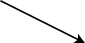
\includegraphics[scale=4.0]{figures/figure-line}
\end{center}


\subsubsection{cArcFigure}

\cclass{cArcFigure} displays an axis-aligned arc. (To display a
non-axis-aligned arc, apply a transform to \cclass{cArcFigure}, or use
\cclass{cPathFigure}.) The arc's geometry is determined by the bounding box
of the circle or ellipse, and a start and end angle; they can be set with
the \ffunc{setBounds()}, \ffunc{setStartAngle()} and \ffunc{setEndAngle()}
methods. Other properties such as color and line style are inherited from
\cclass{cAbstractLineFigure}.

For angles, zero points east. Angles that go counterclockwise are
positive, and those that go clockwise are negative.

\begin{note}
Angles are in radians in the C++ API, but in degrees when the figure is
defined in the NED file via \fprop{@figure}.
\end{note}

Here is an example that draws a blue arc with an arrowhead that goes
counter-clockwise from 3 hours to 12 hours on the clock:

\begin{cpp}
cArcFigure *arc = new cArcFigure("arc");
arc->setBounds(cFigure::Rectangle(100100,50,50));
arc->setStartAngle(0);
arc->setEndAngle(M_PI/2);
arc->setLineColor(cFigure::BLUE);
arc->setEndArrowhead(cFigure::ARROW_BARBED);
\end{cpp}

%% NOTE to authors: code should be kept in sync with test/anim/usman/*.cc!

The result:

\begin{center}

\includegraphics[scale=4.0]{figures/figure-arc}
\end{center}


\subsubsection{cPolylineFigure}

By default, \cclass{cPolylineFigure} displays multiple connecting straight
line segments. The class stores geometry information as a sequence of
points. The line may be \textit{smoothed}, so the figure can also display
complex curves.

The points can be set with \ffunc{setPoints()} that takes \ttt{std::vector<Point>},
or added one-by-one using \ffunc{addPoint()}. Elements in the point list can be
read and overwritten (\ffunc{getPoint()}, \ffunc{setPoint()}). One can also
insert and remove points (\ffunc{insertPoint()} and \ffunc{removePoint()}.

A smoothed line is drawn as a series of Bezier curves, which touch the
start point of the first line segment, the end point of the last line
segment, and the midpoints of intermediate line segments, while
intermediate points serve as control points. Smoothing can be turned on/off
using \ffunc{setSmooth()}.

Additional properties such as color and line style are inherited from
\cclass{cAbstractLineFigure}. Line join style (which is not part of
\cclass{cAbstractLineFigure}) can be set with \ffunc{setJoinStyle()}.

Here is an example that uses a smoothed polyline to draw a spiral:

\begin{cpp}
cPolylineFigure *polyline = new cPolylineFigure("polyline");
const double C=1.1;
for (int i = 0; i < 6; i++)
    polyline->addPoint(cFigure::Point(10*i*cos(C*i), 10*i*sin(C*i)));
polyline->move(100, 100);
polyline->setSmooth(true);
\end{cpp}

%% NOTE to authors: code should be kept in sync with test/anim/usman/*.cc!

The result, with both \textit{smooth=false} and \textit{smooth=true}:

\begin{center}
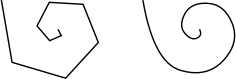
\includegraphics[scale=4.0]{figures/figure-polylines}
\end{center}


\subsubsection{cAbstractShapeFigure}

\cclass{cAbstractShapeFigure} is an abstract base class for various shapes,
providing line and fill color, line and fill opacity, line style, line
width, and other properties for them.

Both outline and fill are optional, they can be turned on and off
independently with the \ffunc{setOutlined()} and \ffunc{setFilled()}
methods. The default is outlined but unfilled shapes.

Similar to \cclass{cAbstractLineFigure}, line color can be set with
\ffunc{setLineColor()}, and line width with \ffunc{setLineWidth()}.
Lines can be solid, dashed, dotted, etc.; line style can be set with
\ffunc{setLineStyle()}. The default fill color is black.

Fill color can be set with \ffunc{setFillColor()}. The default fill color
is blue (although it is indifferent until one calls \ttt{setFilled(true)}).

\begin{note}
Invoking \ffunc{setFillColor()} alone does not make the shape filled,
you also need to call \ffunc{setFilled(true)} for that.
\end{note}

Shapes can be partially transparent, and opacity can be set individually
for the outline and the fill, using \ffunc{setLineOpacity()} and
\ffunc{setFillOpacity()}. These functions accept a \ttt{double} between 0
and 1: a zero argument means fully transparent, and one means fully opaque.

When the outline is drawn with a width larger than one pixel, it will be
drawn symmetrically, i.e. approximately 50-50\% of its width will fall
inside and outside the shape. (This also means that the fill and a wide
outline will partially overlap, but that is only apparent if the
outline is also partially transparent.)

Transformations such as scaling or skew do affect the width of the line as it
is rendered on the canvas. Whether zooming (by the user) should also affect
it can be controlled by setting a flag (\ffunc{setZoomLineWidth()}).
The default is non-zooming lines.

Specifying zero for line width is currently not allowed. The reason is that
it would make sense to display zero-width lines as hairlines that are
always rendered as one pixel wide regardless of transforms and zoom level,
but that is not possible on all platforms.


\subsubsection{cRectangleFigure}

\cclass{cRectangleFigure} displays a rectangle with optionally rounded
corners. As with all shape figures, drawing of both the outline and the
fill are optional. Line and fill color, and several other properties are
inherited from \cclass{cAbstractShapeFigure}.

The figure's geometry can be set with the \ffunc{setBounds()} method that
takes a \cclass{cFigure::Rectangle}. The radii for the rounded corners can
be set independently for the $x$ and $y$ direction using
\ffunc{setCornerRx()} and \ffunc{setCornerRy()}, or together with
\ffunc{setCornerRadius()}.

The following example draws a rounded rectangle of size 80x50, filled with
a "good dark color".

\begin{cpp}
cRectangleFigure *rect = new cRectangleFigure("rect");
rect->setBounds(cFigure::Rectangle(100,100,80,50));
rect->setCornerRadius(5);
rect->setFilled(true);
rect->setFillColor(cFigure::GOOD_DARK_COLORS[0]);
\end{cpp}

%% NOTE to authors: code should be kept in sync with test/anim/usman/*.cc!

The result:

\begin{center}

\includegraphics[scale=4.0]{figures/figure-rectangle}
\end{center}


\subsubsection{cOvalFigure}

\cclass{cOvalFigure} displays a circle or an axis-aligned ellipse. As with
all shape figures, drawing of both the outline and the fill are optional.
Line and fill color, and several other properties are inherited from
\cclass{cAbstractShapeFigure}.

The geometry is specified with the bounding box, and it can be set with the
\ffunc{setBounds()} method that takes a \cclass{cFigure::Rectangle}.

The following example draws a circle of diameter 50 with a wide dotted line.

\begin{cpp}
cOvalFigure *circle = new cOvalFigure("circle");
circle->setBounds(cFigure::Rectangle(100,100,50,50));
circle->setLineWidth(3);
circle->setLineStyle(cFigure::LINE_DOTTED);
\end{cpp}

%% NOTE to authors: code should be kept in sync with test/anim/usman/*.cc!

The result:

\begin{center}
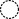
\includegraphics[scale=4.0]{figures/figure-oval}
\end{center}


\subsubsection{cRingFigure}

\cclass{cRingFigure} displays a ring, with explicitly controllable
inner/outer radii. The inner and outer circles (or ellipses) form the
outline, and the area between them is filled. As with all shape figures,
drawing of both the outline and the fill are optional. Line and fill color,
and several other properties are inherited from
\cclass{cAbstractShapeFigure}.

The geometry is determined by the bounding box that defines the outer
circle, and the $x$ and $y$ radii of the inner oval. They can be set with
the \ffunc{setBounds()}, \ffunc{setInnerRx()} and \ffunc{setInnerRy()}
member functions. There is also a utility method for setting both
inner radii together, named \ffunc{setInnerRadius()}.

The following example draws a ring with an outer diameter of 50 and
inner diameter of 20.

\begin{cpp}
cRingFigure *ring = new cRingFigure("ring");
ring->setBounds(cFigure::Rectangle(100,100,50,50));
ring->setInnerRadius(10);
ring->setFilled(true);
ring->setFillColor(cFigure::YELLOW);
\end{cpp}

%% NOTE to authors: code should be kept in sync with test/anim/usman/*.cc!

\begin{center}

\includegraphics[scale=4.0]{figures/figure-ring}
\end{center}


\subsubsection{cPieSliceFigure}

\cclass{cPieSliceFigure} displays a pie slice, that is, a section of an
axis-aligned disc or filled ellipse.  The outline of the pie slice consists
of an arc and two radii. As with all shape figures, drawing of both the
outline and the fill are optional.

Similar to an arc, a pie slice is determined by the bounding box of the
full disc or ellipse, and a start and an end angle. They can be set with
the \ffunc{setBounds()}, \ffunc{setStartAngle()} and \ffunc{setEndAngle()}
methods.

For angles, zero points east. Angles that go counterclockwise are
positive, and those that go clockwise are negative.

\begin{note}
Angles are in radians in the C++ API, but in degrees when the figure is
defined in the NED file via \fprop{@figure}.
\end{note}

Line and fill color, and several other properties are inherited from
\cclass{cAbstractShapeFigure}.

The following example draws pie slice that's one third of a whole pie:

\begin{cpp}
cPieSliceFigure *pieslice = new cPieSliceFigure("pieslice");
pieslice->setBounds(cFigure::Rectangle(100,100,50,50));
pieslice->setStartAngle(0);
pieslice->setEndAngle(2*M_PI/3);
pieslice->setFilled(true);
pieslice->setLineColor(cFigure::BLUE);
pieslice->setFillColor(cFigure::YELLOW);
\end{cpp}

%% NOTE to authors: code should be kept in sync with test/anim/usman/*.cc!

The result:

\begin{center}
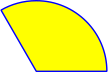
\includegraphics[scale=4.0]{figures/figure-pieslice}
\end{center}


\subsubsection{cPolygonFigure}

\cclass{cPolygonFigure} displays a (closed) polygon, determined by a sequence of points.
The polygon may be \textit{smoothed}. A smoothed polygon is drawn as a series
of cubic Bezier curves, where the curves touch the midpoints of the sides,
and vertices serve as control points. Smoothing can be turned on/off
using \ffunc{setSmooth()}.

The points can be set with \ffunc{setPoints()} that takes \ttt{std::vector<Point>},
or added one-by-one using \ffunc{addPoint()}. Elements in the point list can be
read and overwritten (\ffunc{getPoint()}, \ffunc{setPoint()}). One can also
insert and remove points (\ffunc{insertPoint()} and \ffunc{removePoint()}.

As with all shape figures, drawing of both the outline and the fill
are optional. The drawing of filled self-intersecting polygons is controlled
by the fill rule, which defaults to even-odd (\ttt{FILL\_EVENODD}), and
can be set with \ffunc{setFillRule()}. Line join style can be set with
the \ffunc{setJoinStyle()}.

Line and fill color, and several other properties are inherited from
\cclass{cAbstractShapeFigure}.

Here is an example of a smoothed polygon that also demonstrates
the use of \ffunc{setPoints()}:

\begin{cpp}
cPolygonFigure *polygon = new cPolygonFigure("polygon");
std::vector<cFigure::Point> points;
points.push_back(cFigure::Point(0, 100));
points.push_back(cFigure::Point(50, 100));
points.push_back(cFigure::Point(100, 100));
points.push_back(cFigure::Point(50, 50));
polygon->setPoints(points);
polygon->setSmooth(true);
polygon->setLineColor(cFigure::BLUE);
\end{cpp}

%% NOTE to authors: code should be kept in sync with test/anim/usman/*.cc!

The result, with both \textit{smooth=false} and \textit{smooth=true}:

\begin{center}
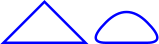
\includegraphics[scale=4.0]{figures/figure-polygons}
\end{center}


\subsubsection{cPathFigure}

\cclass{cPathFigure} displays a "path", a complex shape or line modeled after SVG
paths. A path may consist of any number of straight line segments, Bezier
curves and arcs. The path can be disjoint as well. Closed paths may be filled.
The drawing of filled self-intersecting polygons is controlled by the
\textit{fill rule} property. Line and fill color, and several other properties
are inherited from \cclass{cAbstractShapeFigure}.

A path, when given as a string, looks like this one that draws a triangle:

\textit{M 150 0 L 75 200 L 225 200 Z}

It consists of a sequence of commands (\textit{M} for \textit{moveto},
\textit{L} for \textit{lineto}, etc.) that are each followed by numeric
parameters (except \textit{Z}). All commands can be expressed with
lowercase letter, too. A capital letter means that the target point is
given with \textit{absolute} coordinates, a lowercase letter means they are
given \textit{relative} to the target point of the previous command.

\cclass{cPathFigure} can accept the path in string form (\ffunc{setPath()}),
or one can assemble the path with a series of method calls like
\ffunc{addMoveTo()}. The path can be cleared with the \ffunc{clearPath()}
method.

The commands with argument list and the corresponding \textit{add} methods:

\begin{itemize}
\item \tbf{M} \textit{x y}: move; \ffunc{addMoveTo()}, \ffunc{addMoveRel()}
\item \tbf{L} \textit{x y}: line; \ffunc{addLineTo()}, \ffunc{addLineRel()}
\item \tbf{H} \textit{x}: horizontal line; \ffunc{addHorizontalLineTo()}, \ffunc{addHorizontalLineRel()}
\item \tbf{V} \textit{y}: vertical line; \ffunc{addVerticalLineTo()}, \ffunc{addVerticalLineRel()}
\item \tbf{A} \textit{rx ry phi largeArc sweep x y}: arc; \ffunc{addArcTo()}, \ffunc{addArcRel()}
\item \tbf{Q} \textit{x1 y1 x y}: curve; \ffunc{addCurveTo()}, \ffunc{addCurveRel()}
\item \tbf{T} \textit{x y}: smooth curve; \ffunc{addSmoothCurveTo()}, \ffunc{addSmoothCurveRel()}
\item \tbf{C} \textit{x1 y1 x2 y2 x y}: cubic Bezier curve; \ffunc{addCubicBezierCurveTo()}, \ffunc{addCubicBezierCurveRel()}
\item \tbf{S} \textit{x2 y2 x y}: smooth cubic Bezier curve; \ffunc{addSmoothCubicBezierCurveTo()}, \ffunc{addSmoothCubicBezierCurveRel()}
\item \tbf{Z}: close path; \ffunc{addClosePath()}
\end{itemize}

In the parameter lists, $(x,y)$ are the target points (substitute $(dx,dy)$ for
the lowercase, relative versions.) For the Bezier curves, $x1,y1$ and
$(x2,y2)$ are control points. For the arc, $rx$ and $ry$ are the radii of the
ellipse, $phi$ is a rotation angle in degrees for the ellipse, and
$largeArc$ and $sweep$ are both booleans (0 or 1) that select which portion
of the ellipse should be taken.\footnote{For more details, consult the SVG
specification.}

No matter how the path was created, the string form can be obtained with the
\ffunc{getPath()} method, and the parsed form with the \ffunc{getNumPathItems()},
\ffunc{getPathItem(k)} methods. The latter returns pointer to a
\cclass{cPathFigure::PathItem}, which is a base class with subclasses for every
item type.

Line join style, cap style (for open subpaths), and fill rule (for closed
subpaths) can be set with the \ffunc{setJoinStyle()},
\ffunc{setCapStyle()}, \ffunc{setFillRule()} methods.

\cclass{cPathFigure} has one more property, a $(dx,dy)$ offset, which
exists to simplify the implementation of the \ffunc{move()} method. Offset
causes the figure to be translated by the given amount for drawing. For
other figure types, \ffunc{move()} directly updates the coordinates, so it
is effectively a wrapper for \ffunc{setPosition()} or \ffunc{setBounds()}.
For path figures, implementing \ffunc{move()} so that it updates every path
item would be cumbersome and potentially also confusing for users. Instead,
\ffunc{move()} updates the offset. Offset can be set with
\ffunc{setOffset()},

In the first example, the path is given as a string:

%% TODO example that draws several disjoint items in one path: a rect, zigzag curve, etc.

\begin{cpp}
cPathFigure *path = new cPathFigure("path");
path->setPath("M 0 150 L 50 50 L 100 150 Z");
path->setFilled(true);
path->setLineColor(cFigure::BLUE);
path->setFillColor(cFigure::YELLOW);
\end{cpp}

%% NOTE to authors: code should be kept in sync with test/anim/usman/*.cc!

The second example creates the equivalent path programmatically.

\begin{cpp}
cPathFigure *path = new cPathFigure("path");
path->addMoveTo(0,150);
path->addLineTo(50,50);
path->addLineTo(100,150);
path->addClosePath();
path->setFilled(true);
path->setLineColor(cFigure::BLUE);
path->setFillColor(cFigure::YELLOW);
\end{cpp}

%% NOTE to authors: code should be kept in sync with test/anim/usman/*.cc!

The result:

TODO

\subsubsection{cAbstractTextFigure}

\cclass{cAbstractTextFigure} is an abstract base class for figures that
display (potentially multi-line) text.

The location of the text on the canvas is determined jointly by a
\textit{position} and an \textit{anchor}. The anchor tells how to
place the text relative to the positioning point. For example,
if anchor is \ttt{ANCHOR\_CENTER} then the text is centered on the point;
if anchor is \ttt{ANCHOR\_N} then the text will be drawn so that its top
center point is at the positioning point. The values
\ttt{ANCHOR\_BASELINE\_START}, \ttt{ANCHOR\_BASELINE\_MIDDLE},
\ttt{ANCHOR\_BASELINE\_END} refer to the beginning, middle and end of the
baseline of the (first line of the) text as anchor point. The member
functions to set the positioning point and the anchor are
\ffunc{setPosition()} and \ffunc{setAnchor()}. Anchor defaults to
\ttt{ANCHOR\_CENTER}.

The font can be set with the \ffunc{setFont()} member function that takes
\cclass{cFigure::Font}, a class that encapsulates typeface, font style and
size. Color can be set with \ffunc{setColor()}. The displayed text can
also be partially transparent. This is controlled with the \ffunc{setOpacity()}
member function that accepts an \ttt{double} in the $[0,1]$ range, $0$ meaning
fully transparent (invisible), and $1$ meaning fully opaque.


\subsubsection{cTextFigure}

\cclass{cTextFigure} displays text which is affected by zooming and
transformations. Font, color, position, anchoring and other properties are
inherited from \cclass{cAbstractTextFigure}.

The following example displays a text in dark blue 12-point bold Arial
font.

\begin{cpp}
cTextFigure *text = new cTextFigure("text");
text->setText("This is some text.");
text->setPosition(cFigure::Point(100,100));
text->setAnchor(cFigure::ANCHOR_BASELINE_MIDDLE);
text->setColor(cFigure::Color("#000040"));
text->setFont(cFigure::Font("Arial", 12, cFigure::FONT_BOLD));
\end{cpp}

%% NOTE to authors: code should be kept in sync with test/anim/usman/*.cc!

The result:

\begin{center}

\includegraphics[scale=4.0]{figures/figure-text}
\end{center}


\subsubsection{cLabelFigure}

\cclass{cLabelFigure} displays text which is unaffected by zooming or
transformations, except its position. Font, color, position, anchoring and
other properties are inherited from \cclass{cAbstractTextFigure}.

The following example displays a label in Courier New with the default
size, slightly transparent.

\begin{cpp}
cLabelFigure *label = new cLabelFigure("label");
label->setText("This is a label.");
label->setPosition(cFigure::Point(100,100));
label->setAnchor(cFigure::ANCHOR_NW);
label->setFont(cFigure::Font("Courier New"));
label->setOpacity(0.9);
\end{cpp}

%% NOTE to authors: code should be kept in sync with test/anim/usman/*.cc!

The result:

\begin{center}
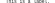
\includegraphics[scale=4.0]{figures/figure-label}
\end{center}


\subsubsection{cAbstractImageFigure}

\cclass{cAbstractImageFigure} is an abstract base class for image figures.

The location of the image on the canvas is determined jointly by a
\textit{position} and an \textit{anchor}. The anchor tells how to
place the image relative to the positioning point. For example,
if anchor is \ttt{ANCHOR\_CENTER} then the image is centered on the point;
if anchor is \ttt{ANCHOR\_N} then the image will be drawn so that its top
center point is at the positioning point. The member functions to set the
positioning point and the anchor are \ffunc{setPosition()} and
\ffunc{setAnchor()}. Anchor defaults to \ttt{ANCHOR\_CENTER}.

By default, the figure's width/height will be taken from the image's
dimensions in pixels. This can be overridden with the\ffunc{setWidth()} /
\ffunc{setHeight()} methods, causing the image to be scaled.
\ttt{setWidth(0)} / \ttt{setHeight(0)} reset the default (automatic) width
and height.

One can choose from several interpolation modes that control how the image
is rendered when it is not drawn in its natural size. Interpolation mode
can be set with \ffunc{setInterpolation()}, and defaults to
\ttt{INTERPOLATION\_FAST}.

Images can be tinted; this feature is controlled by a tint color and a tint
amount, a $[0,1]$ real number. They can be set with the
\ffunc{setTintColor()} and \ffunc{setTintAmount()} methods, respectively.

Images may also be rendered as partially transparent, which is controlled by
the opacity property, a $[0,1]$ real number. Opacity can be set with the
\ffunc{setOpacity()} method. The rendering process will combine this
property with the transparency information contained within the image, i.e.
the alpha channel.


\subsubsection{cImageFigure}

\cclass{cImageFigure} displays an image, typically an icon or a background
image, loaded from the {\opp} image path. Positioning and other properties
are inherited from \cclass{cAbstractImageFigure}. Unlike \cclass{cIconFigure},
\cclass{cImageFigure} fully obeys transforms and zoom.

The following example displays a map:

\begin{cpp}
cImageFigure *image = new cImageFigure("map");
image->setPosition(cFigure::Point(0,0));
image->setAnchor(cFigure::ANCHOR_NW);
image->setImageName("maps/europe");
image->setWidth(600);
image->setHeight(500);
\end{cpp}

%% NOTE to authors: code should be kept in sync with test/anim/usman/*.cc!


\subsubsection{cIconFigure}

\cclass{cIconFigure} displays a non-zooming image, loaded from the {\opp}
image path. Positioning and other properties are inherited from
\cclass{cAbstractImageFigure}.

\cclass{cIconFigure} is not affected by transforms or zoom, except its position.
(It can still be resized, though, via \ffunc{setWidth()} / \ffunc{setHeight()}.)

The following example displays an icon similar to the way the
\ttt{"i=block/sink,gold,30"} display string tag would, and makes
it slightly transparent:

\begin{cpp}
cIconFigure *icon = new cIconFigure("icon");
icon->setPosition(cFigure::Point(100,100));
icon->setImageName("block/sink");
icon->setTintColor(cFigure::Color("gold"));
icon->setTintAmount(0.3);
icon->setOpacity(0.8);
\end{cpp}

%% NOTE to authors: code should be kept in sync with test/anim/usman/*.cc!

The result:

\begin{center}

\includegraphics[scale=4.0]{figures/figure-icon}
\end{center}


\subsubsection{cPixmapFigure}

\cclass{cPixmapFigure} displays a user-defined raster image. A pixmap
figure may be used to display e.g. a heat map. Support for scaling and
various interpolation modes are useful here. Positioning and other
properties are inherited from \cclass{cAbstractImageFigure}.

A pixmap itself is represented by the \cclass{cFigure::Pixmap} class.

\cclass{cFigure::Pixmap} stores a rectangular array of 32-bit RGBA pixels,
and allows pixels to be manipulated directly. The size ($width \times
height$) as well as the default fill can be specified in the constructor.
The pixmap can be resized (i.e. pixels added/removed at the right and/or bottom)
using \ffunc{setSize()}, and it can be filled with a color using \ffunc{fill()}.
Pixels can be directly accessed with \ffunc{pixel(x,y)}.

A pixel is returned as type \cclass{cFigure::RGBA}, which is a convenience
struct that, in addition to having the four public \ttt{uint8\_t} fields
(\ttt{red}, \ttt{green}, \ttt{blue}, \ttt{alpha}), is augmented with several
utility methods.

Many \cclass{Pixmap} and \cclass{RGBA} have methods that
accept or return \cclass{cFigure::Color} and opacity, converting between
them and RGBA. (Opacity is a $[0,1]$ real number that is mapped to the
0..255 alpha channel.)

One can set up and manipulate the image that \cclass{cPixmapFigure} display
in two ways. First, one can create and fill a \cclass{cFigure::Pixmap}
separately, and set it on \cclass{cPixmapFigure} using \ffunc{setPixmap()}.
This will overwrite the figure's internal pixmap instance that it displays.
The second way is to utilize \cclass{cPixmapFigure}'s methods such as
\ffunc{setSize()}, \ffunc{fill()}, \ffunc{setSize()}, \ffunc{setPixel()},
\ffunc{setPixelColor()}, \ffunc{setPixelOpacity()}, etc. that delegate to
the internal pixmap instance.

TODO setWidth() / setHeight() vs setPixmapSize()!

The following example displays a heat map by manipulating the transparency
of the pixels:

TODO refresh code!

\begin{cpp}
cPixmapFigure *pixmapFigure = new cPixmapFigure("pixmap");
pixmapFigure->setPosition(cFigure::Point(100,100));
pixmapFigure->setWidth(100);
pixmapFigure->setHeight(100); //TODO why there is no setSize() method????
pixmapFigure->setSize(20, 20, cFigure::YELLOW, 1);
for (int y = 0; y < pixmapFigure->getHeight(); y++) {
    for (int x = 0; x < pixmapFigure->getWidth(); x++) {
        double opacity = 1 - sqrt((x-10)*(x-10)/100.0 + (y-10)*(y-10)/100.0);
        pixmapFigure->setPixelOpacity(x, y, opacity);
    }
}
\end{cpp}

%% NOTE to authors: code should be kept in sync with test/anim/usman/*.cc!

The result:

\begin{center}

\includegraphics[scale=4.0]{figures/figure-pixmap}
\end{center}


\subsubsection{cGroupFigure}

\cclass{cGroupFigure} is for the sole purpose of grouping its children. It
has no visual appearance. The usefulness of a group figure comes from the
fact that elements of a group can be hidden / shown together, and also
transformations are inherited from parent to child, thus, children of a
group can be moved, scaled, rotated, etc. together by updating the group's
transformation matrix.

The following example creates a group with two subfigures, then moves and
rotates them as one unit.

\begin{cpp}
cGroupFigure *group = new cGroupFigure("group");

cImageFigure *image = new cImageFigure("img");
image->setPosition(cFigure::Point(0,0));
image->setAnchor(cFigure::ANCHOR_S);
image->setImageName("block/sink");

cLineFigure *line = new cLineFigure("line");
line->setStart(cFigure::Point(-50,10));
line->setEnd(cFigure::Point(50,10));

group->addFigure(image);
group->addFigure(line);
group->translate(100, 100);
group->rotate(M_PI/6, 100, 100);
\end{cpp}

%% NOTE to authors: code should be kept in sync with test/anim/usman/*.cc!

The result:

\begin{center}

\includegraphics[scale=4.0]{figures/figure-group}
\end{center}


\subsection{Compound Figures}

There are two ways the set of figure type can be extended:

\begin{enumerate}
  \item Compound figures.
  \item New standalone figure types
\end{enumerate}

Compound figures are useful when the graphical presentation of a simulation
grows complex, and it becomes desirable to be able to group certain figures
into larger units that can be created and manipulated like a single figure.

Such compound figures can be created by subclassing e.g. \cclass{cGroupFigure}.
The constructor would create and add subfigures as children, and also remember
their pointers. Added getter and setter methods would delegate to subfigures.

%% TODO example: change the cGroupFigure example to be a subclass of cGroupFigure

\subsection{Defining New Figure Types}

It is is more difficult to create new figure types where the rendering is not
based on already existing figures. The difficulty arises from the point that
figures are only data storate classes, actual drawing takes place in the
GUI library such as Tkenv and Qtenv. Thus, it is not enough to write the new
figure class itself, but one also needs to extend Tkenv and/or Qtenv as well,
to add the rendering code.

We won't go into full details of how to extend Tkenv/Qtenv here, just give
you a few pointers in case you need it.

In both Tkenv and Qtenv, rendering is done with the help of figure renderer
classes that have a class hierarchy roughly parallel to the
\cclass{cFigure} inheritance tree. The base classes are incidentally called
\cclass{FigureRenderer}. How figure renderers do their job is different in
Tkenv and Qtenv: in Tkenv, rendering occurs by creating and maintaining
canvas items on a Tkpath canvas; on Qtenv, they create and manipulate
\cclass{QGraphicsItem}s on a \cclass{QGraphicsView}. To be able to render a
new figure type, one needs to create the appropriate figure renderer
classes for Tkenv, Qtenv, or both.

The names of the renderer classes are provided by the figures themselves,
by their \ffunc{getRendererClassName()} methods. For example,
\cclass{cLineFigure}'s \ffunc{getRendererClassName()} returns
\ttt{LineFigureRenderer}. Qtenv qualifies that with its own namespace, and
looks for a registered class named
\ttt{omnetpp::qtenv::LineFigureRenderer}. If such class exists and is a
Qtenv figure renderer (the appropriate \ttt{dynamic\_cast} succeeds), an
instance of that class will be used to render the figure, otherwise an
error message will be issued. Tkenv does something similar.


\section{3D Visualization}
\label{sec:ch-graphics:osg}

\subsection{Introduction}

{\opp} lets one build advanced 3D visualization for simulation models.
3D visualization is useful for wide range of simulations, including
mobile wireless networks, transportation models, factory floorplan
simulations and more. One can visualize terrain, roads, urban street
networks, indoor environments, satellites, and more. It is possible to
augment the 3D scene with various annotations. For wireless network
simulations, for example, one can create a scene that, in addition to
the faithful representation of the physical world, also displays the
transmission range of wireless nodes, their connectivity graph
and various statistics, indicates individual wireless transmissions
or traffic intensity, and so on.

In {\opp}, 3D visualization is completely distinct from display
string-based and canvas-based visualization. The scene appears on a
separate GUI area. Visualizing 3D scenes is currently only supported
in Qtenv (i.e. it is unavailable in Tkenv.)

{\opp}'s 3D visualization is based on the open-source OpenSceneGraph
and osgEarth libraries. These libraries offer high-level functionality,
such as the ability of using 3D model files directly, accessing and
rendering online map and satellite imagery data sources, and so on.

\subsubsection{OpenSceneGraph and osgEarth}

OpenSceneGraph (openscenegraph.org), or OSG for short, is the base library.
It is best to quote their web site:

\begin{displayquote}
"OpenSceneGraph is an open source high performance 3D graphics toolkit,
used by application developers in fields such as visual simulation, games,
virtual reality, scientific visualization and modeling. Written entirely in
Standard C++ and OpenGL, it runs on all Windows platforms, OS X, GNU/Linux,
IRIX, Solaris, HP-UX, AIX and FreeBSD operating systems. OpenSceneGraph is
now well established as the world leading scene graph technology, used
widely in the vis-sim, space, scientific, oil-gas, games and virtual
reality industries."
\end{displayquote}

In turn, osgEarth (osgearth.org) is a geospatial SDK and terrain engine built on top
of OpenSceneGraph, not quite unlike Google Earth. It has many attractive features:

\begin{itemize}
\item Able to use various street map providers, satellite imaging providers,
      altitude data sources, both online and offline
\item Data from online sources may be exported into a file suitable for offline use
\item Scene may be annotated with various types of graphical objects
\item Includes conversion between various geographical coordinate systems
\end{itemize}

On the basic level, osgEarth is very easy to use. To get started, one only
needs to create a simple XML file, and point it at the appropriate map data
source.

\subsection{Building 3D Visualization}

For 3D visualization, {\opp} basically exposes the OpenSceneGraph API.
You assemble an OSG scene graph in the model, and give it to {\opp} for
display. The scene graph can be updated at runtime, and changes will be
reflected in the display.

\begin{note}
\tbf{What is a scene graph?} A scene graph is a tree-like directed graph
data structure that describes a 3D scene. The root node represents the
whole virtual world. The world is then broken down into a hierarchy of
nodes representing either spatial groupings of objects, settings of
the position of objects, animations of objects, or definitions of
logical relationships between objects. The leaves of the graph
represent the physical objects themselves, the drawable geometry and
their material properties.
\end{note}

When a scene graph has been built in the model, it needs to be given
to a \cclass{cOsgCanvas} object to let the {\opp} GUI know about it.
\cclass{cOsgCanvas} wraps a scene graph, plus hints for the GUI
on how to best display the scene, for example the default camera
position. In the GUI, the user can use the mouse to manipulate the
camera to view the scene from the various angles and distances, look
at various parts of the scene, and so on.

It is important to note that the simulation model may only directly
manipulate the scene graph, but it cannot directly access the viewer
in the GUI. The viewer is inaccessible, and may not be directly
manipulated. There is a very specific technical reason for that.
The viewer may not even exist or may be displaying a different
scene graph at the time the model tries to access it. The model
may even be running under a non-GUI user interface (e.g. Cmdenv)
where a viewer is not even part of the program. The viewer may
only be influenced in the form of viewer hints in
\cclass{cOsgCanvas}.


\subsubsection{Creating and Accessing cOsgCanvas Objects}

Every module has a built-in (default) \cclass{cOsgCanvas}, which can be
accessed with the \ffunc{getOsgCanvas())} method of \cclass{cModule}.
For example, a toplevel submodule can get hold of the network's
OSG canvas with the following line:

\begin{cpp}
cOsgCanvas *osgCanvas = getParentModule()->getOsgCanvas();
\end{cpp}

Additional \cclass{cOsgCanvas} instances may be created simply with \ttt{new}:

\begin{cpp}
cOsgCanvas *osgCanvas = new cOsgCanvas("scene2");
\end{cpp}

\subsubsection{cOsgCanvas and Scene Graphs}

Once a scene graph has been assembled, it can be set on \cclass{cOsgCanvas}
with the \ffunc{setScene()} method.

\begin{cpp}
osg::Node *scene = ...
osgCanvas->setScene(scene);
\end{cpp}

Subsequent changes in the scene graph will be automatically reflected in
the visualization, there is no need to call \ffunc{setScene()} again or
otherwise let {\opp} know about the changes.


\subsubsection{Viewer Hints}

There are several hints that the 3D viewer may take into account when displaying
the scene graph. Note that hints are only hints, so the viewer may choose to
ignore them, and the user may also be able to override them interactively,
(using the mouse, via the context menu, hotkeys or by other means).

The viewer style can be set with \ffunc{setViewerStyle()}. Choices are
\ttt{STYLE\_GENERIC} that should be set for generic (non-osgEarth) scenes,
and \ttt{STYLE\_EARTH} for osgEarth scenes.

The OSG viewer makes uses of camera manipulators that map mouse and keyboard
gestures to camera movement. The preferred camera manipulator can
be set with \ffunc{setCameraManipulatorType()} that takes an enum.
Several camera manipulators are available:

\begin{itemize}
\item \ttt{CAM\_TRACKBALL} works best for viewing floating 3D objects from all directions
\item \ttt{CAM\_EARTH} is intended for Earth scenes
\item \ttt{CAM\_TERRAIN} is similar to \ttt{CAM\_EARTH}?? TODO
\item \ttt{CAM\_OVERVIEW} is TODO
\item \ttt{CAM\_AUTO} selects the best option based on other settings and the model. This is the default.
\end{itemize}

\ffunc{setClearColor()}

\ffunc{setFieldOfViewAngle()}

\ffunc{setZNear()}

\ffunc{setZFar()}

Set all perspective-related viewer hints together:
\ffunc{setPerspective()} takes fieldOfViewAngle, zNear and zFar together

\ffunc{setGenericViewpoint()} takes \cclass{cOsgCanvas::Viewpoint}

\ffunc{setEarthViewpoint()} takes \cclass{osgEarth::Viewpoint}


\begin{cpp}
osgCanvas->setViewerStyle(cOsgCanvas::STYLE_EARTH);
\end{cpp}


\subsubsection{Making Nodes Clickable}

TODO

\subsubsection{Conditional compilation}

Model code should surround OSG-specific code with \fmac{\#ifdef HAVE\_OSG}.

A complete example:

\begin{cpp}
#include <osgDB/ReadFile>
#include <omnetpp.h>
...
TODO #ifdef HAVE_OSG
void DemoModule::initialize()
{
    cOsgCanvas *osgCanvas = getParentModule()->getOsgCanvas();
    osg::Node *scene = ... // assemble scene graph here
    osgCanvas->setScene(scene);
    osgCanvas->setClearColor(cOsgCanvas::Color(0,0,64)); // hint
}
\end{cpp}


\subsection{Practical Advice to 3D Visualization}

there are numerous sources to get information and practical help in using OSG.

the intent of the next sections is just to give you enough material to get started.

after that you are advised to refer to the material listed in the section "OSG programming resources"

\subsubsection{Loading Models}

To display a 3D model in the canvas of a compound module, an \cclass{osg::Node} has
to be provided as the root of the scene.

One method of getting such a \ttt{Node} is to load it from a file containing the
model. [1]

This can be done with the \ffunc{osgDB::readNodeFile()} method (or with one
of its variants). This method takes a string as argument, and based on the
protocol specification and extension(s), finds a suitable loader for it,
loads it, finally returns with a pointer to the newly created \cclass{osg::Node}
instance. [2]

This node can now be set on the canvas for display with the \ffunc{setScene()}
method, as seen in the osg-intro sample (among others):

\begin{cpp}
osg::Node *model = osgDB::readNodeFile("model.osgb");
getParentModule()->getOsgCanvas()->setScene(model);
\end{cpp}

\begin{note}
\tbf{Where to get model files?} While OpenSceneGraph recognizes and can
load a wide range of formats, many 3D modeling tools can also export the
edited scene or part of it in OSG's native file format, osgt, with the
help of exporter plugins. One such plugin for Blender has been used to
develop some of the OSG demos for {\opp}, and it was found to be working
well. [3]
\end{note}

There is support for so-called "pseudo loaders" in OSG, which provide
additional options for loading models. Those allow for some basic
operations to be performed on the model after it is loaded. To use them,
simply append the parameters for the modifier followed by the name of it to
the end of the file name upon loading the model.

Take this line from the osg-earth sample for example:

\begin{inifile}
*.cow[*].modelURL = "cow.osgb.2.scale.0,0,90.rot.0,0,-15e-1.trans"
\end{inifile}

This string will first scale the original cow model in \ttt{cow.osgb} to
200\%, then rotate it 90 degrees around the Z axis and finally translate it
1.5 units downwards. The floating point numbers have to be represented in
scientific notation to avoid the usage of decimal points or commas in the
number as those are already used as operator and parameter separators.

Note that these modifiers operate directly on the model data and are
independent of any further dynamic transformations applied to the node when
it is placed in the scene. For further information refer to the OSG
knowledge base. [4]

\subsubsection{Building the Scene}

Alternatively, the whole scene can be built entirely from scratch using the
\cclass{osg::Geode}, \cclass{osg::ShapeDrawable} and \cclass{osg::Shape}
classes. This eliminates the need for separate model files in the
simulation.

For an example of this see the Satellite.cc file in the osg-satellites
sample:

\begin{cpp}
auto cone = new osg::Cone(osg::Vec3(0, 0, -coneRadius*0.75), coneHeight, coneRadius);
auto coneDrawable = new osg::ShapeDrawable(cone);
auto coneGeode = new osg::Geode;
coneGeode->addDrawable(coneDrawable);
locatorNode->addChild(coneGeode);
\end{cpp}

Independent of how the scene has been constructed, it is always important
to keep track of how the individual nodes are related to each other in the
scene graph. This is because every modification of an osg::Node is by
default propagated to all of its children, let it be a transformation, a
render state variable, or some other flag.

For really simple scenes it might be enough to have an osg::Group as the
root node, and make every other object a direct child of that. This reduces
the complications and avoids any strange surprises regarding state
inheritance. For more complex scenes it is advisable to follow the logical
hierarchy of the displayed objects in the scene graph.

Once the desired object is created and added to the scene, it can be easily
moved and oriented to represent the state of the simulation by making it a
child of an osg::PositionAttitudeTransform node.

\subsubsection{Earth Files}

TODO example: substitute "boston.earth"


\subsubsection{Transforms}

TODO

\subsubsection{Animation Playback}

For more sophisticated animation it is also possible to play back stored
motion sequences from the model file, as seen in the osg-indoor sample or
the BostonPark scenario of the osg-earth sample. The former demonstrates
explicit control over which animation is being played when and in what way,
while the latter contains a really simple looping clip (the box people)
requiring no control from the model code.

\subsubsection{Earth Files}

When using the Earth-style viewer for a module, the displayed globe is
specified by a .earth file. This can be as simple as a single image
textured over a sphere or as complex as realistic terrain data and
satellite images complete with street and building information dynamically
streamed over the internet from a publicly available provider, thanks to
the flexibility of osgEarth. For more information on .earth files see the
reference [5] or one of the sample simulations.

To place objects on the terrain easily, using natural geographic coordinate
systems, the osgEarth::Util::ObjectLocatorNode can be used, as seen in the
osg-satellites sample for instance.

\subsubsection{Looking at the Sample Simulations}

TODO

[1]: http://trac.openscenegraph.org/projects/osg//wiki/Support/Tutorials/FileLoadingAndTransforms
[2]: http://trac.openscenegraph.org/projects/osg//wiki/Support/UserGuides/Plugins
[3]: https://github.com/cedricpinson/osgexport
[4]: http://trac.openscenegraph.org/projects/osg//wiki/Support/KnowledgeBase/PseudoLoader
[5]: http://docs.osgearth.org/en/latest/references/earthfile.html


\subsection{OpenSceneGraph Programming Resources}

\subsubsection{Online resources}

TODO

\subsubsection{Books}

The following OpenSceneGraph books have been available at the time of writing:

\begin{itemize}
\item \textit{OpenSceneGraph Quick Start Guide}, by Paul Martz.

This book is a concise introduction to the OpenSceneGraph API. It can be
purchased from http://www.osgbooks.com, and it is also available as
a free pdf download.

\item \textit{OpenSceneGraph 3.0: Beginners Guide}, by Wang Rui. Packt Publishing, 2010.

This book is a concise introduction to the main features of OpenSceneGraph
which then leads you into the fundamentals of developing virtual reality
applications. Practical instructions and explanations accompany you every
step of the way.

\item \textit{OpenSceneGraph 3.0 Cookbook}, by Wang Rui and Qian Xuelei. Packt Publishing, 2010.

This book contains 100 recipes in 9 chapters, focusing on different
fields including the installation, nodes, geometries, camera manipulation,
animations, effects, terrain building, data management, GUI integration.

\end{itemize}


%%% Local Variables:
%%% mode: latex
%%% TeX-master: "usman"
%%% End:

